%======================================================================
%===  dtuposter - a class to make posters tha comply with the DTU CI
%
% Written and maintained in 2011-2014 
% by Jorrit Wronski (jowr@mek.dtu.dk)
%
%
%==========================================
%===  details and poster setup
\documentclass[
%    ,title     = {{Title test}}
%    ,author    = {{ThisIs MyName}}
%    ,subject   = {{This is the subject of my work}}
%    ,bgcolor   = dtulightgreen
%    ,highlight = dtuyellow
%    ,toplogo   = {{tex_dtu_aqua_b_uk}}
%    ,botlogo   = {{tex_dtu_bibliotek_b_uk}}
%    ,papersize = {{a0paper}}
%    ,colcount  = {{1column}}
%    ,longtitle
%    ,largecaption
%    ,draft
%    ,nocrop
%    ,english        % language
%    ,fleqn          % equations on the left
]{dtuposter}
%
%
%======================================================================
%===  Continue with packages
\usepackage[T1]{fontenc}        % special characters
%
%\usepackage[ansinew]{inputenc}  % Windows
%\usepackage[applemac]{inputenc} % MacOS
\usepackage[utf8x]{inputenc}    % Unicode, Linux
%
% 
%======================================================================
%=== Font definitions, DTU recommends Arial for posters
\usepackage{cmbright}
\usepackage{arevmath}
%\usepackage[scaled]{uarial} %Arial clone, set as default sf font - use "ua1" for direct access
%\usepackage{uarial} %Arial clone, set as default sf font - use "ua1" for direct access
%\usepackage[typeface=default,
%            sanstypeface=urwarial,
%            mathtypeface=arevmath
%           ]{typeface}
\renewcommand{\familydefault}{\sfdefault}
\usepackage{enumitem}
\setlist{nosep,leftmargin=*}
%
% 
%======================================================================
%=== Other useful packages
\usepackage{booktabs}
\usepackage{siunitx}
\usepackage{hyperref}
%
% 
%======================================================================
%=== The actual content starts here
\begin{document}

%\begin{itemize}
%\item \texttt{title     = \{\{fine\}\}}
%\item \texttt{author    = \{\{This Ismyname\}\}}
%\item \texttt{subject   = \{\{Subject of the Poster\}\}}
%\item \texttt{bgcolor   = \{\{dtucoolgrey\}\}}
%\item \texttt{highlight = \{\{dtured\}}
%\item \texttt{toplogo   = \{\{tex\_dtu\_mekanik\_b\_uk\}}
%\item \texttt{botlogo   = \{\{tex\_dtu\_elektro\_b\_uk\}\}}
%\item \texttt{papersize = \{\{a0paper\}\}}
%\item \texttt{colcount  = \{\{3columns\}\}}
%\end{itemize}
%
%
%======================================================================
%===  Make header for poster (title and authors)
\begin{dtuposterhead} 
\dtuposterauthor{Jianyi Li\textsuperscript{1}, Xinxing Yu\textsuperscript{1}, Haoyang Liu\textsuperscript{1},  Zhewei Su\textsuperscript{1}}
\dtuposteraffil{\textsuperscript{1} Macau University of Science and Technology, Faculty of Innovation Engineering, Macau, China}

\end{dtuposterhead}
%
%
%======================================================================
%===  ... and the rest of the content
\begin{dtupostercontent}
\section{Introduction}
Chest CT is proved to have a high sensitive in COVID-19 detecting, for the typical radiological features in CT slices. The symptoms include ground-glass opacities, multifocal patchy consolidation and so on. Combining with CT examination, clinic can improve the sensitive of examination and cut down the spreading out at an early stage. Deep learning gets several outbreaks in computer vision area and many algorithms are submitted in medical imaging process. The machine learning models in COVID-19 radiological imaging area are mostly about lesion division. AI assisted medical image process can decrease the workload of clinician and cut off the spread at the early stage.  
\par{
To better accomplish the value of algorithms in real scenario, we want to develop useful software. We expect it to have a high sensitive as well as accuracy, also be easy to use. After developing for nearly one semester, we finally finish our work.
 }

\section{Changelog}
We have published our version 1.0 on report 2. In this new version, we add a label broad for clinician. Also, we fix some bugs assisted in the mainboard. In version 1 we find that the image cannot change with selection box. I will begin on how can we use it, so let’s begin!
\par{After log in, the user will enter such a main board. As our website is design for segmentation, the user can check the CT slices in here and give out auto-segmentation result.}
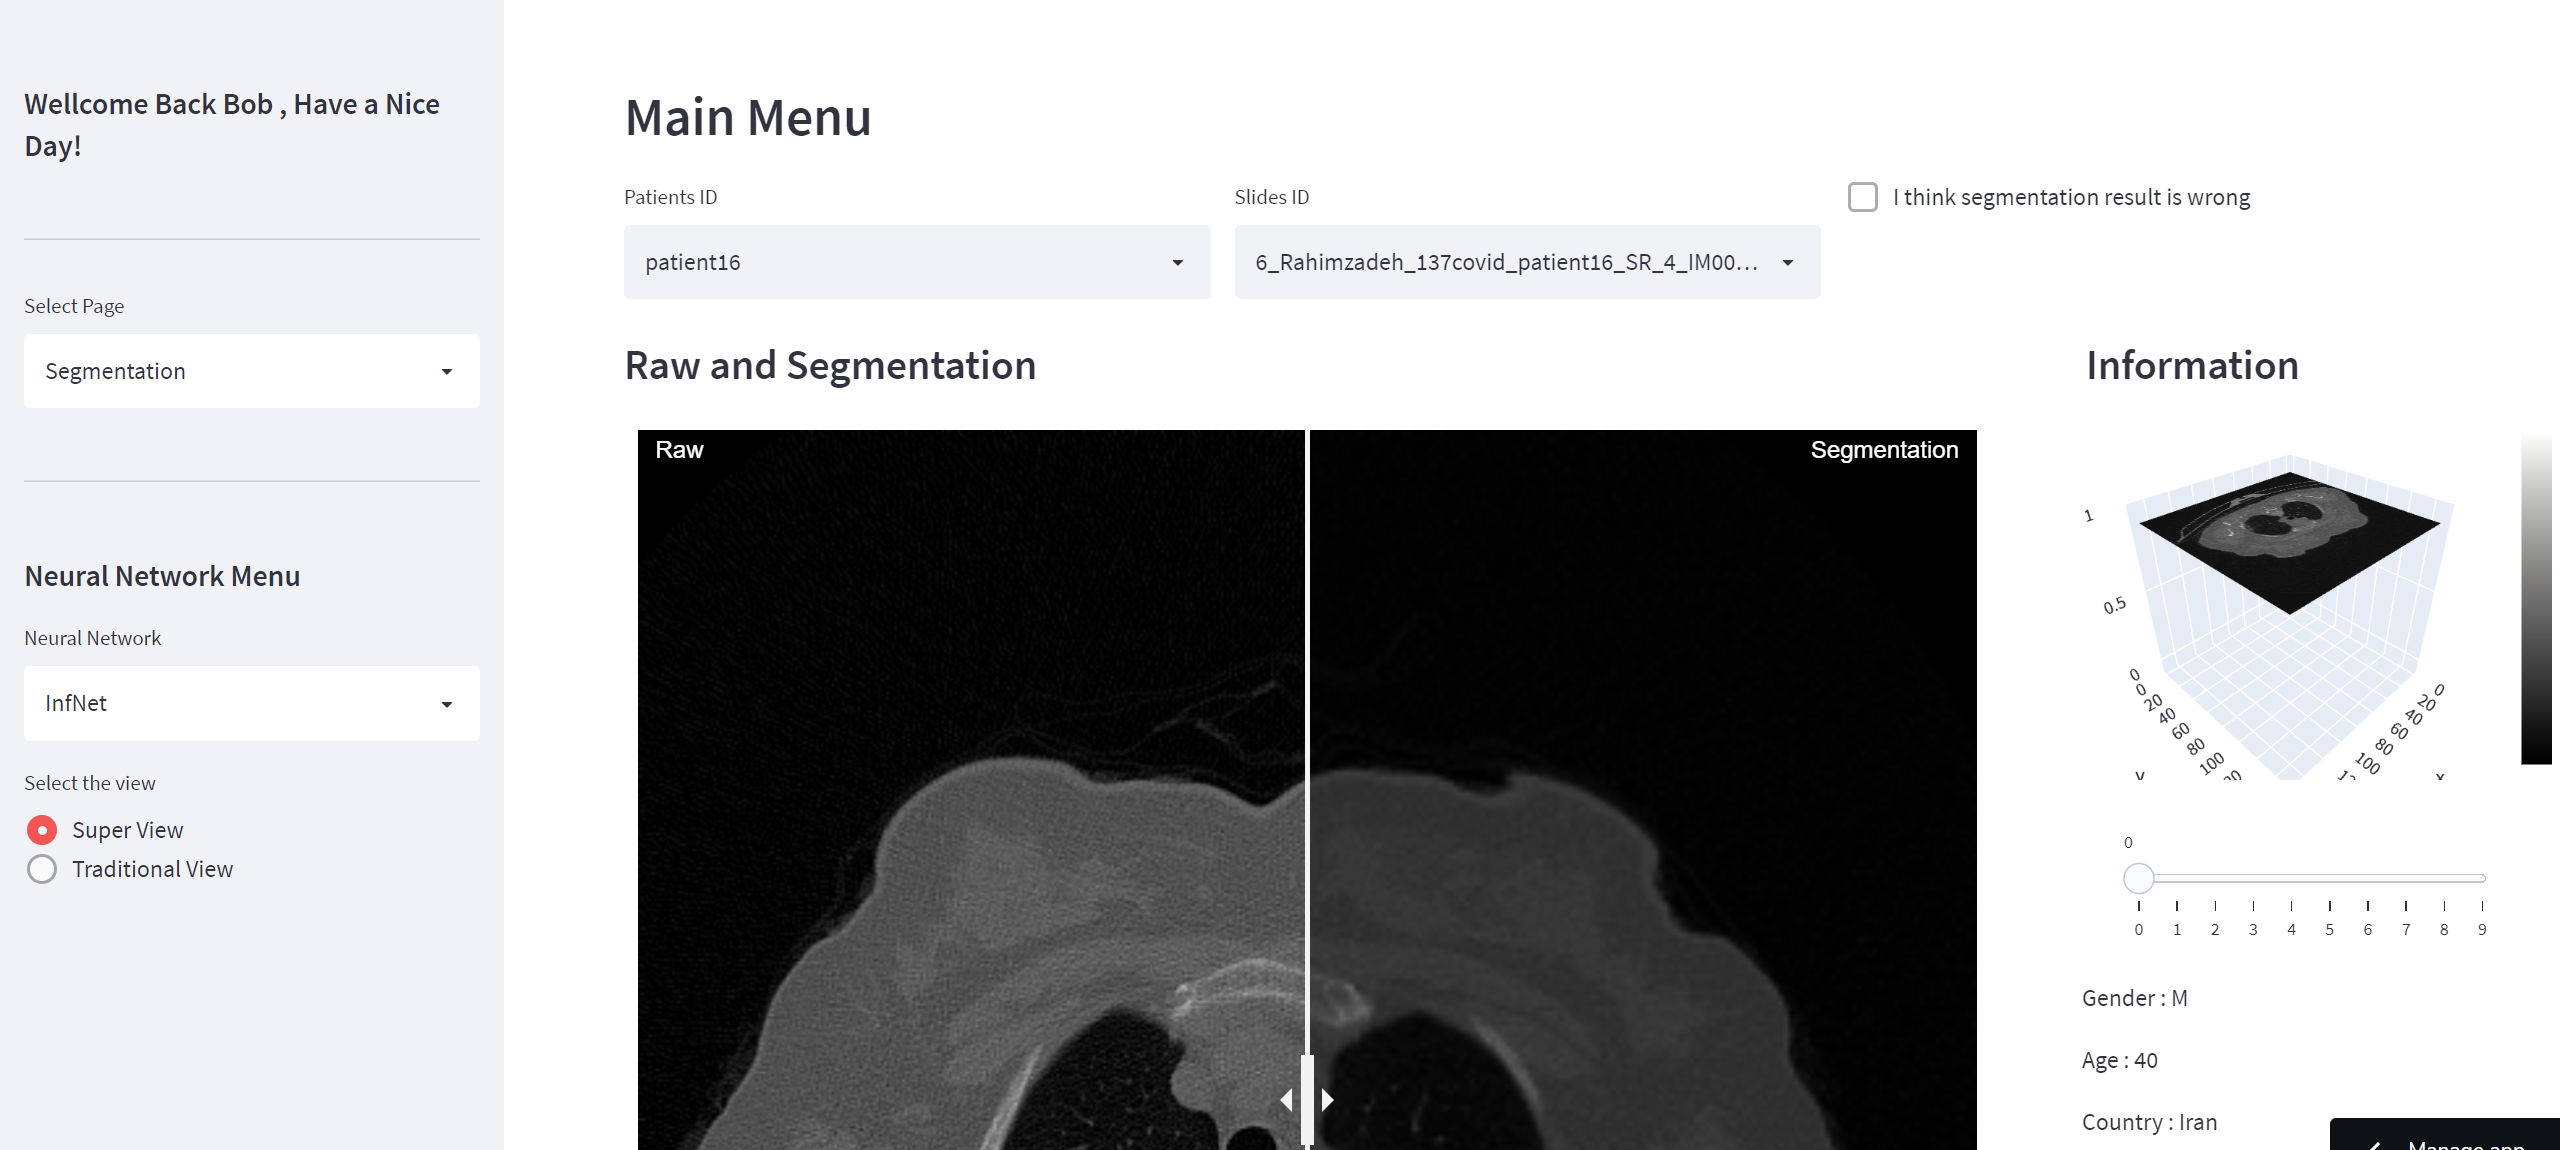
\includegraphics[width=1\linewidth, origin=c]{external/figure/mainbox.png}
\par{In this page we provide 2 user interfaces. One is a traditional view and another is a super view. Here we use super view for example. You can also change the interfaces in the sidebar.}
\begin{figure}
    \centering
\includegraphics[width=.5\linewidth, origin=c]{external/figure/viewselec.png}
\end{figure}
\par{You can change the CT slices with different patients by using the selection box on the top of the page. In version 1.0, we find that the image cannot change with selection box. Therefore, we fix it in this version. In this time, you can get timely feedback of segmentation. You can also change the model. }
\begin{figure}
    \centering
\includegraphics[width=\linewidth, origin=c]{external/figure/changingbutton.png}
\end{figure}
\par{The CT slices are arranged by group using the patient id and the timestamp. In the same group, by dragging the bar below the image, you can change to any other slices. We also provide a 3D indicator. With the change of image, it also give out timely reaction.}
\begin{figure}
    \centering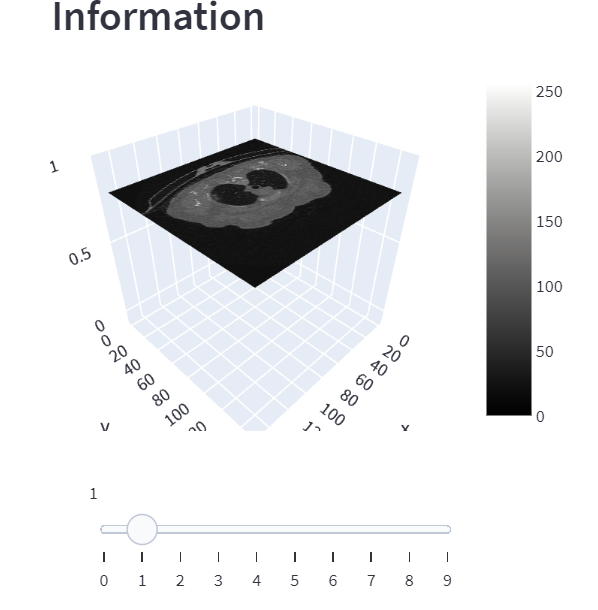
\includegraphics[width=.5\linewidth,origin=c]{external/figure/3dindicator.png}
\end{figure}
\par{the information of patients is print on the right. Detail information including gender, age, country, date and the institution. An auto-diagnosis result is also provided.}
\begin{figure}
    \centering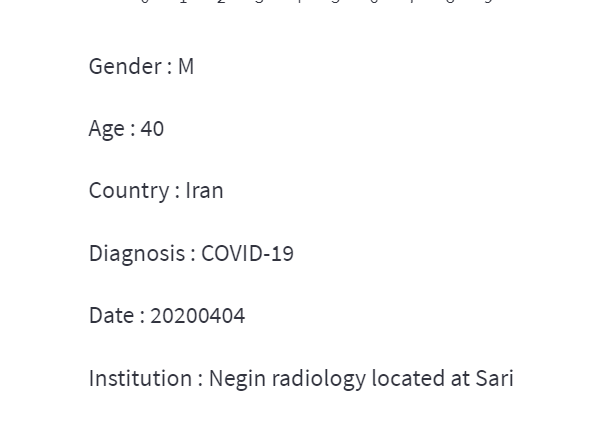
\includegraphics[width=.5\linewidth,origin=c]{external/figure/patientinformation.png}
\end{figure}
\par{After segmentation, you can give out the report of patients. We provide a texting area. After finishing the radiological report, you can click the submit button and finial it will submit to the database.}
\begin{figure}
    \centering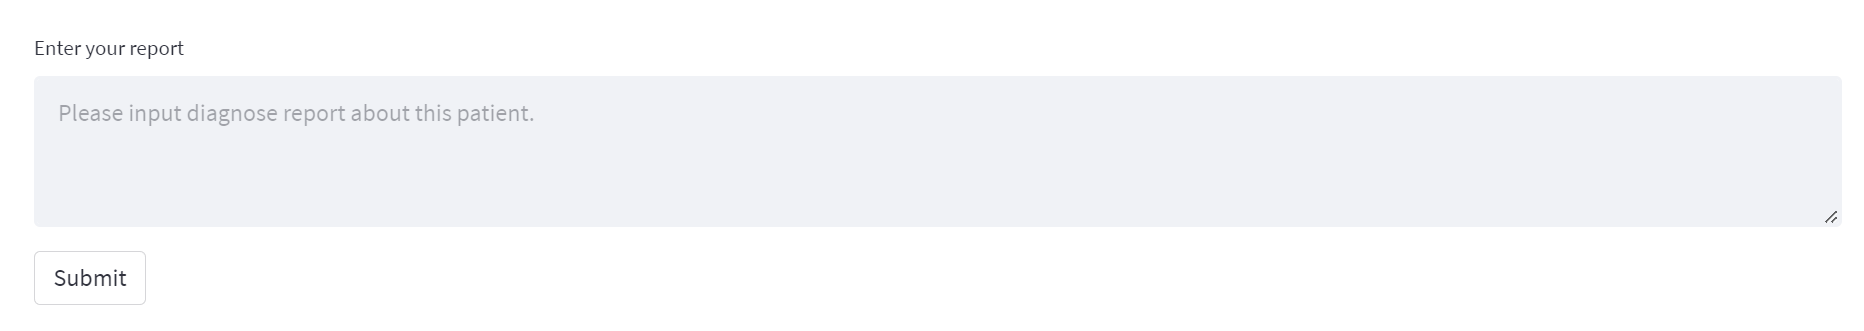
\includegraphics[width=.8\linewidth,origin=c]{external/figure/report.png}
\end{figure}
\par{Definitely, sometime the auto-segmentation result may make mistake. In this version we provide a label board for clinician to change it. If you are not satisfy with the result, click here.}
\begin{figure}
    \centering
\includegraphics[width=.5\linewidth,origin=c]{external/figure/changingbutton.png}
\end{figure}
\par{Then you may get into the label board.We provide 4 ways for the labeling. You can change it in the sidebar. 
In the polygon mode, you can click it to create a point. After selecting all the area, finish selection by click the right mouse button. The design of this is inspired by the lasso tool we use in Photoshop.
You can withdraw the operation by click the button. We also provide a download section.
}
\begin{figure}
    \centering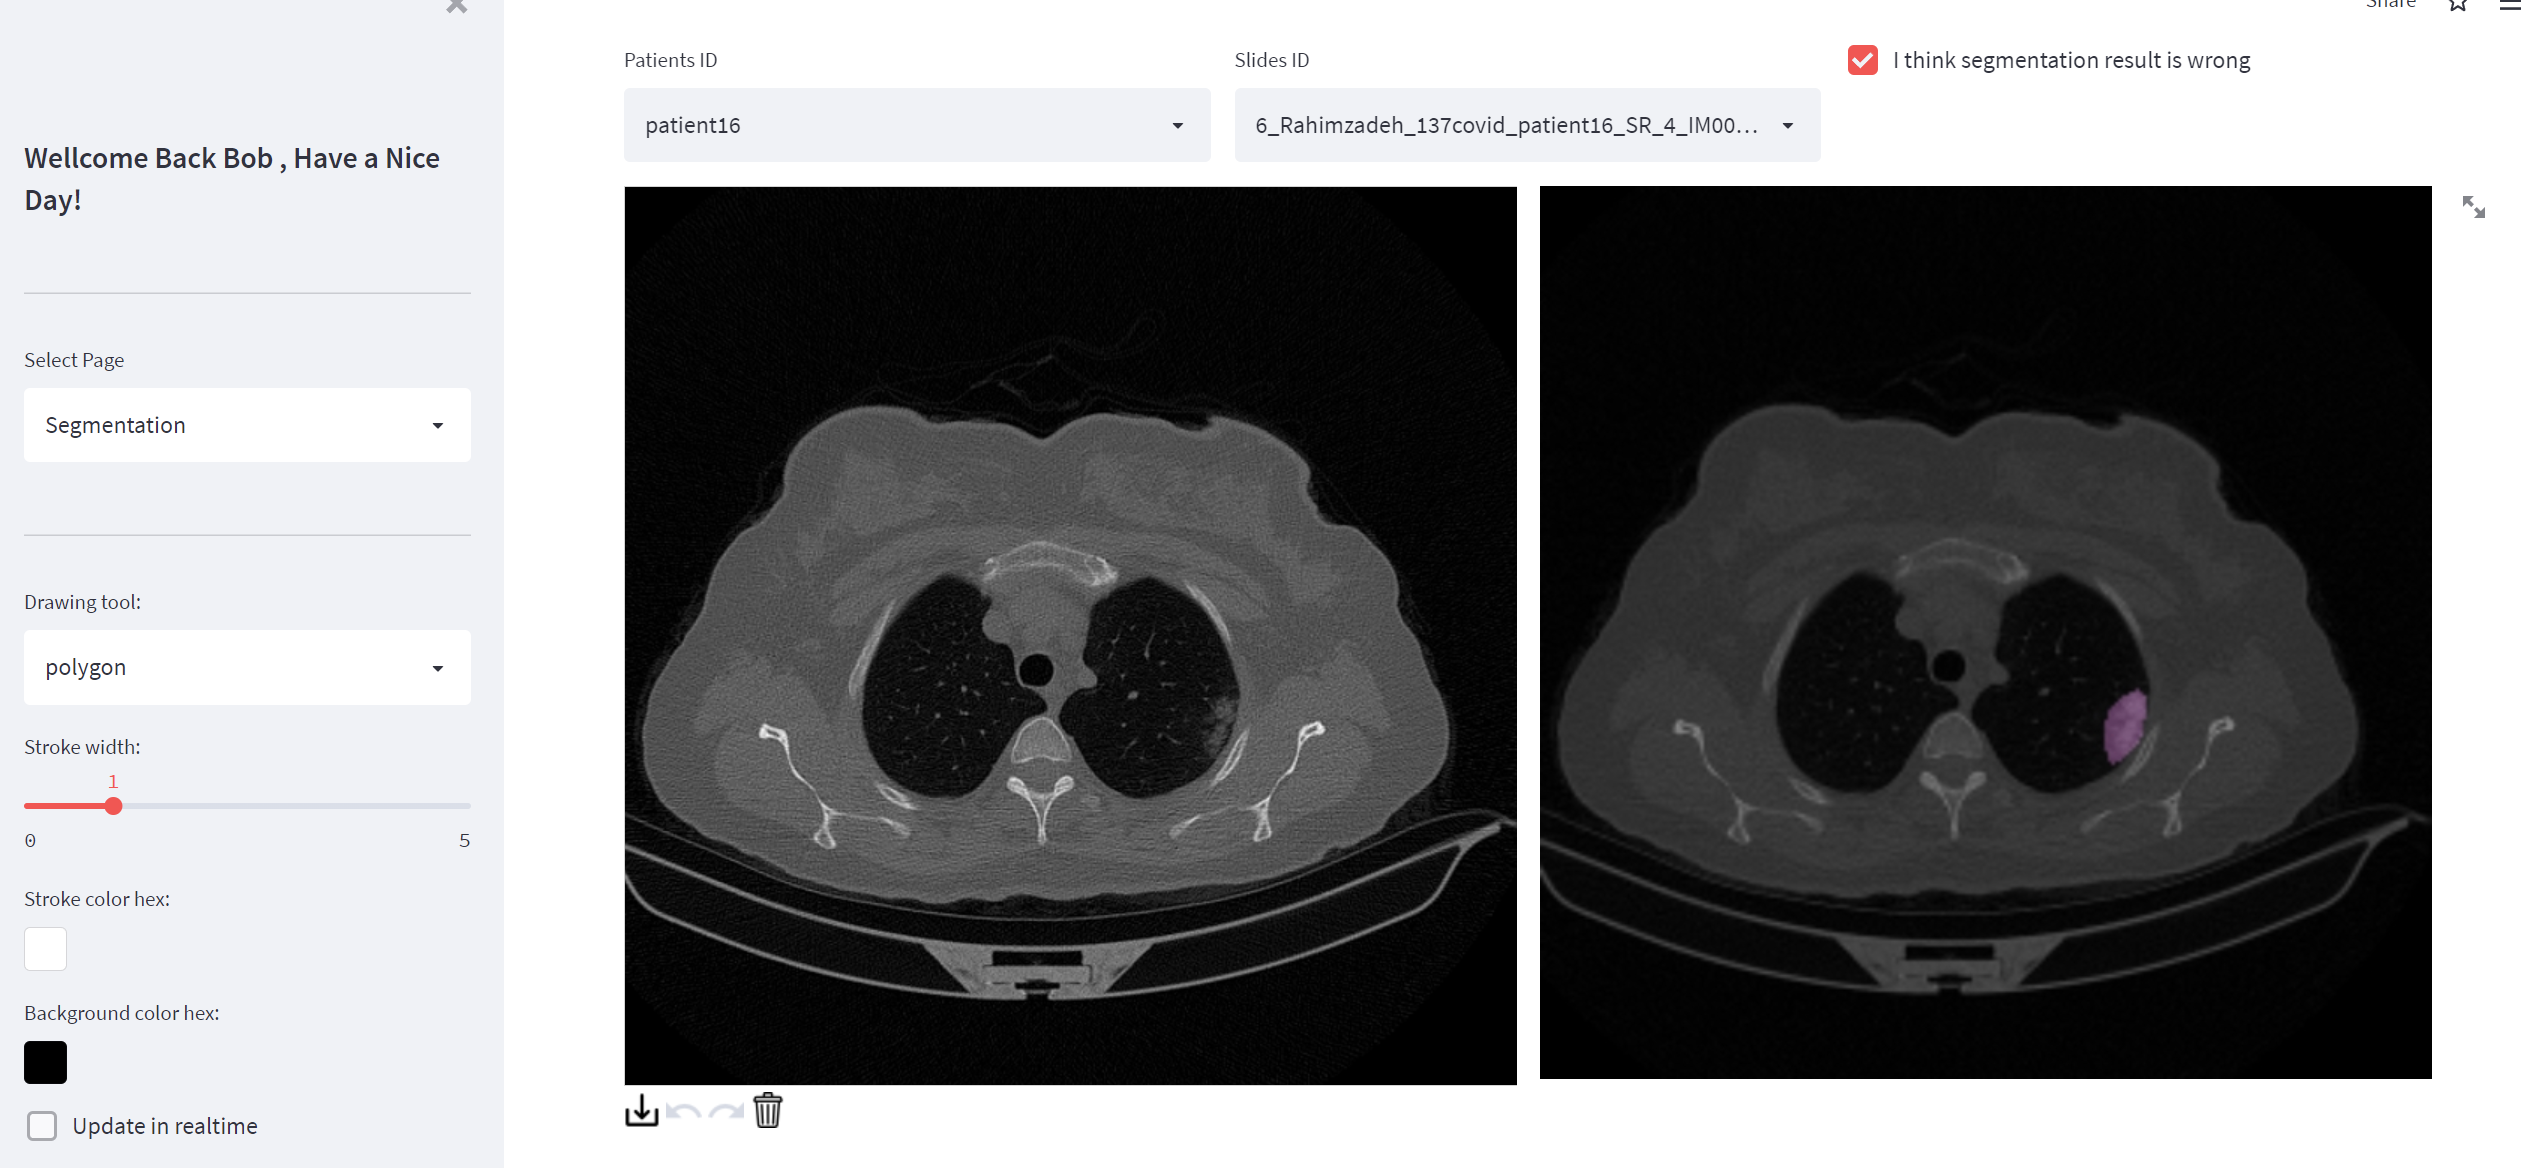
\includegraphics[width=1\linewidth,origin=c]{external/figure/label board.png}
\end{figure}
\par{We also create a patient board, by logging in the website, patient can get their own radiological report and the segmentation result.}

% section2
\section{Workflow}
Here we contain the workflow of our project. A Cumulative flow diagram is used to describe it. Please check our appendix and csv file for more details. 
\begin{figure}
    \centering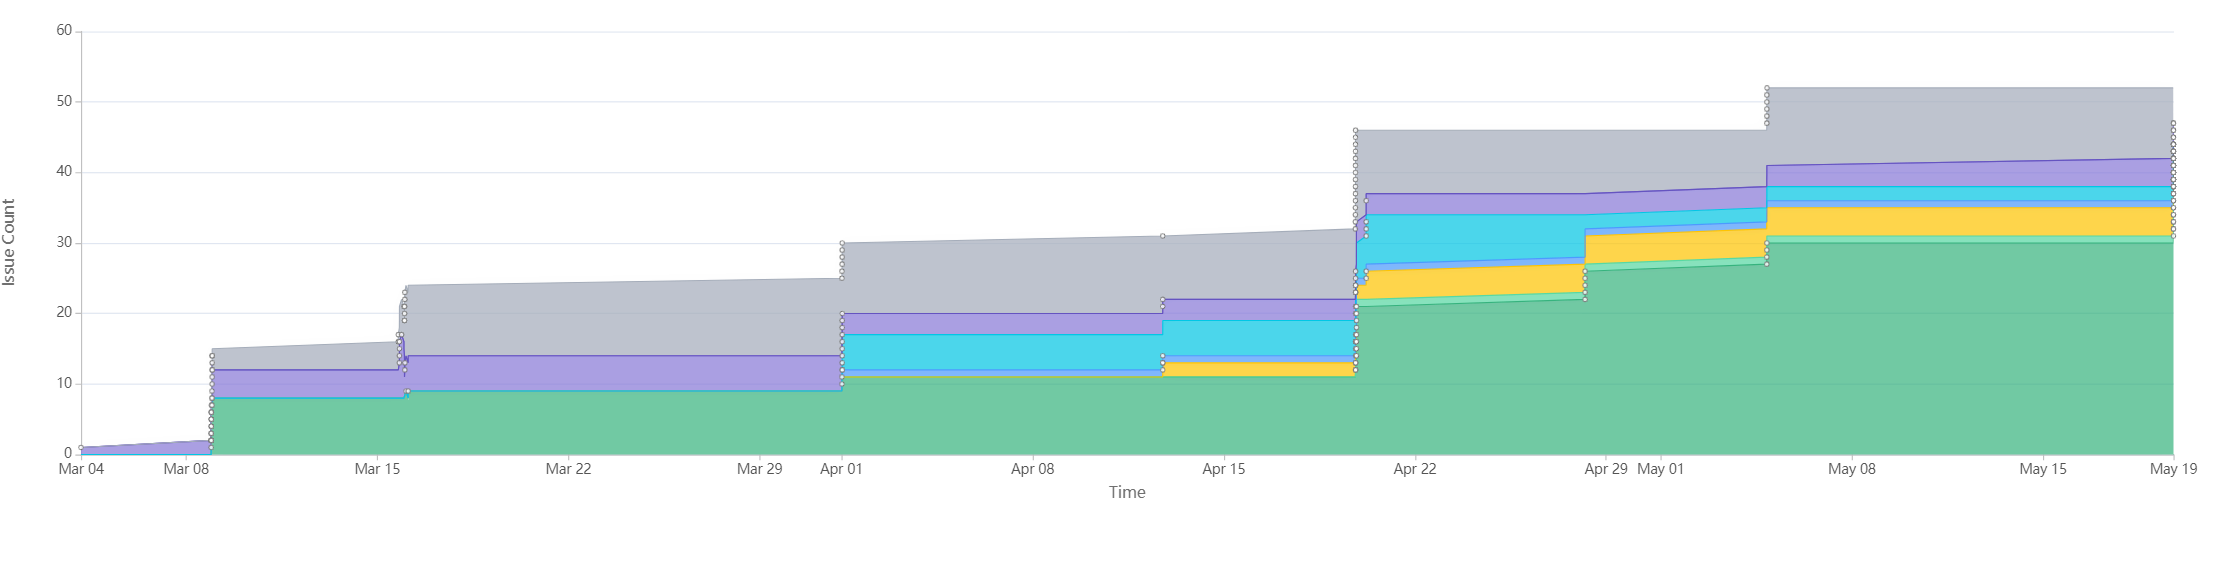
\includegraphics[width=1\linewidth,origin=c]{external/figure/burndownchart.png}
\end{figure}
During the development, we always update Jira after a period of time, this also bring problems as:
\begin{itemize}
    \item [*] There are many platforms in our workflow chart.
    \item [*] The feedback of our project always has delay.
    \item [*] Due to the delay, we repeated in replenishing our documents instead of finish it in time. Therefore, documents may fail to record some bug and loopholes and it may be hard for us to fix the bugs.
\end{itemize}
This really brings trouble to our development. 
\par For the version of software produce, we use to update a version before having the report. Here we shows the board of our sprint 3, and the board of releasing a version as well.
\begin{figure}
    \centering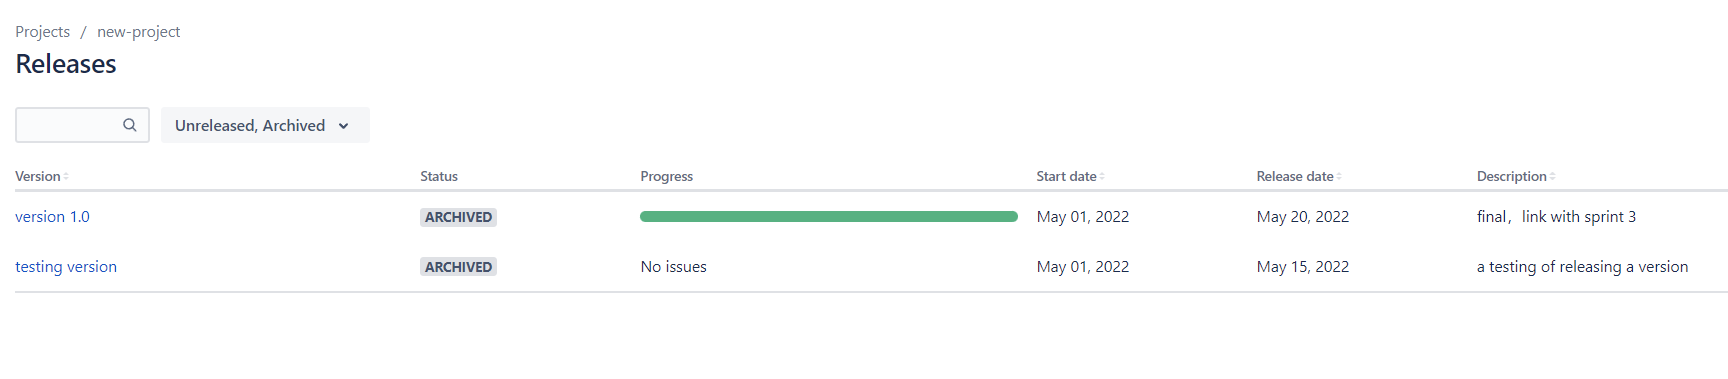
\includegraphics[width=1\linewidth,origin=c]{external/figure/versionrelease.png}
\end{figure}
\begin{figure}
    \centering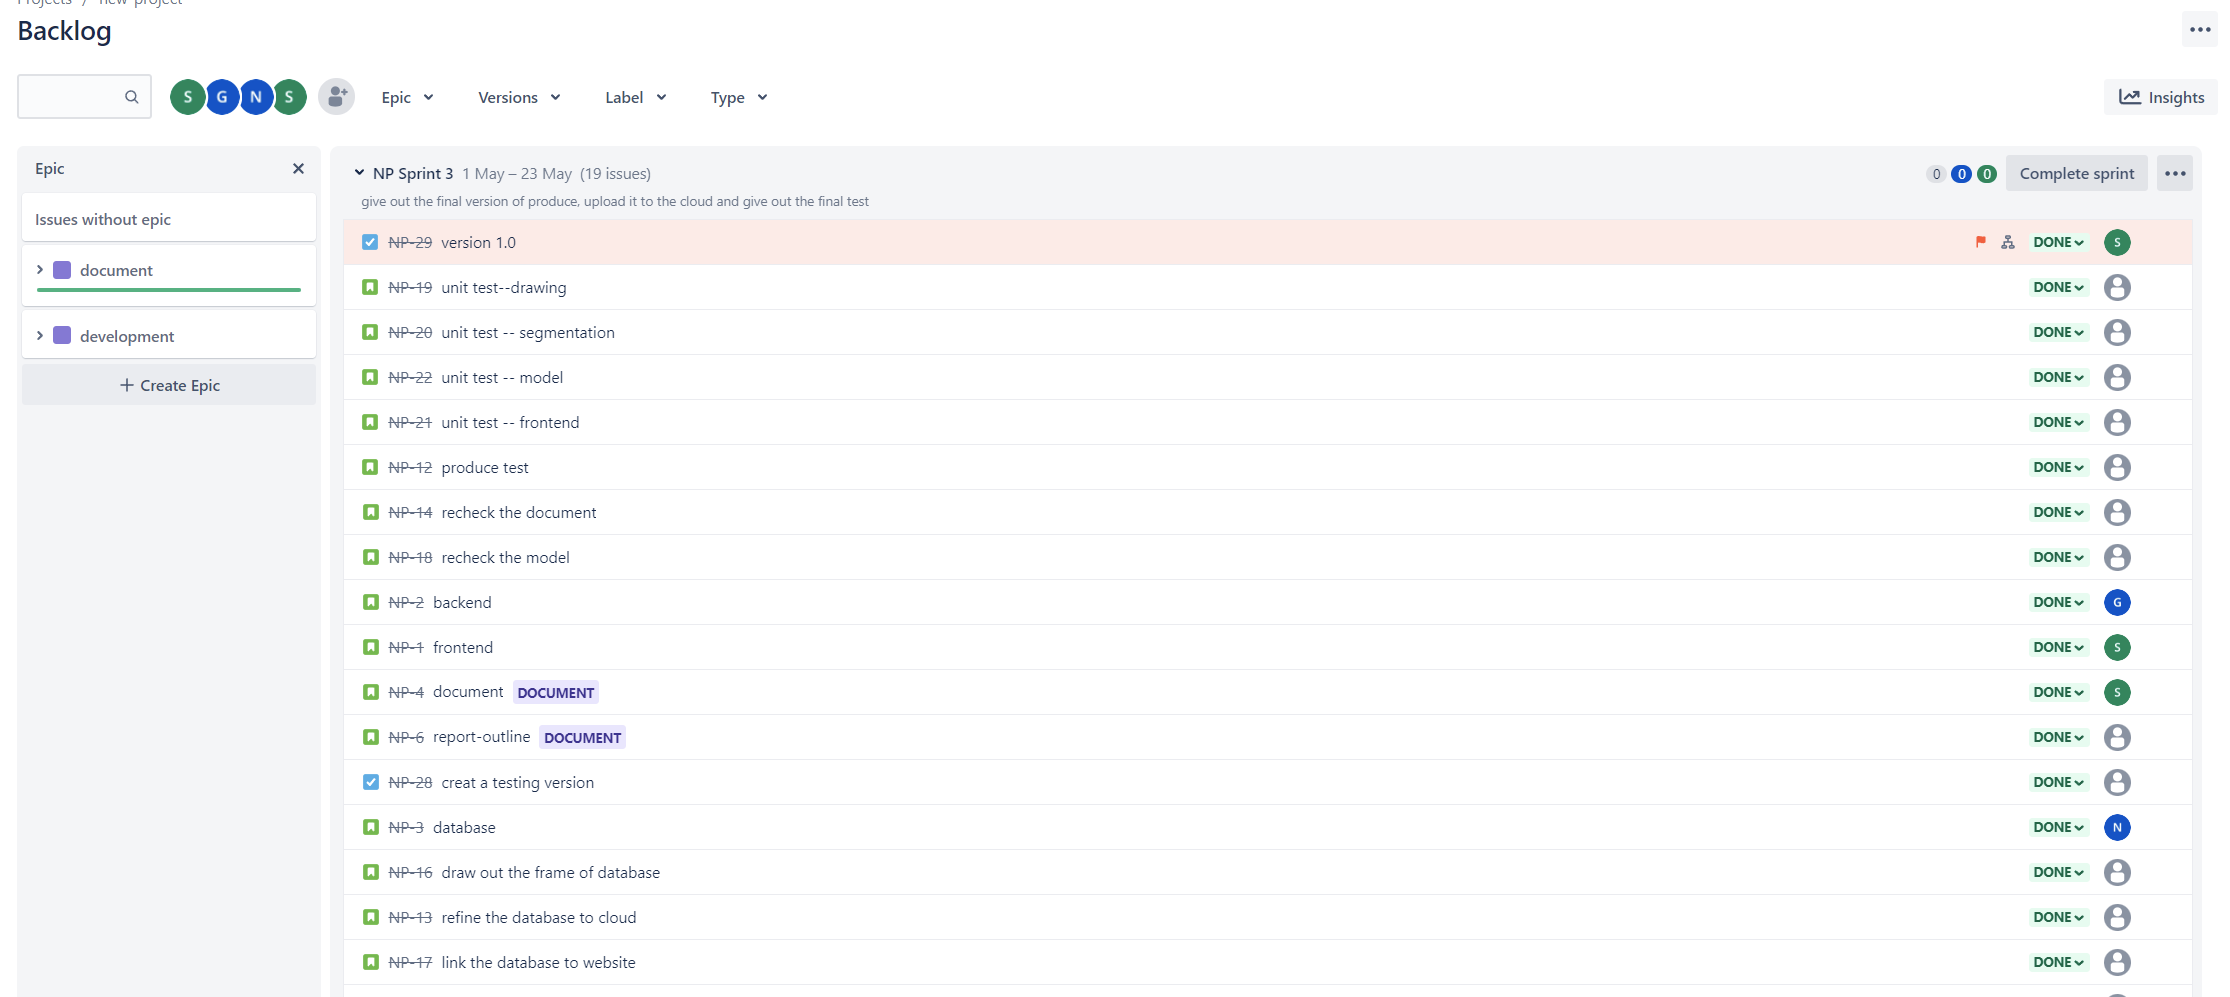
\includegraphics[width=1\linewidth,origin=c]{external/figure/sprint3.png}
\end{figure}
For our source code, please visit our github. (\href{https://github.com/DCTyxx/SegLung}{https://github.com/DCTyxx/SegLung}) We also send a copy without data and DL model in our homework files. You can check the zip file.

% 前景和展望
\section{Loopholes and future work}
Though we finish our developing, we still find much shortage of our product. However, as it comes to the end of semester, we have less time than we thought. Therefore we can only fix some essential bugs of the website. Streamlit only provide 1G memory for free, so we may find it a little stuck for using. Extremely after we add more functions in it.We also finish the example of test, while we did not have time to accomplish it. 
\par For further developing, a database is necessary. We have apply a database in Azure, but due to the time we did not optimize it well. Also the framework of our source code should be optimizing. 
\par Thought there are many dissatisfaction of our project, we exert ourselves in the development. Both of us have learn a lot. It may have pity in our project, but we are satisfied with our workload.
\end{dtupostercontent}

\end{document}
